% \textbf{\underline{OZ 2 - Magnetische velden - Oefening 2:}}
% \vspace{0.5cm}

% Een deeltje met lading $ +q $ en massa $ m $ beweegt in een  uniform magneetveld $ \vec{B} = B_0 \hat{k} $. Op tijdstip $ t = 0 $ is de snelheid van het deeltje gelijk aan $ v_0 $ en de snelheidsvector ligt in het xy-vlak, en maakt een positieve hoek van $ 30^{\circ} $ ten opzichte van de y-as. Op een later tijdstip $ t = t_a $ zal het deeltje de x-as snijden op $ x = a $. In functie van $ q $, $ m $, $ v_0 $ en $ B_0 $, bepaal (a) $ a $, en (b) $ t_a $.

% \begin{description}[labelwidth=1.5cm, leftmargin=!]
%     \item[Geg. :]   $ Q = +q $; $ m $; $ \vec{B} = B_0 \hat{k} $; $ t_0 \Rightarrow v_0 $; $ t_0 \Rightarrow \theta_0 = 30^{\circ} $;
% \end{description}

% \begin{figure}[H]
%     \centering
%     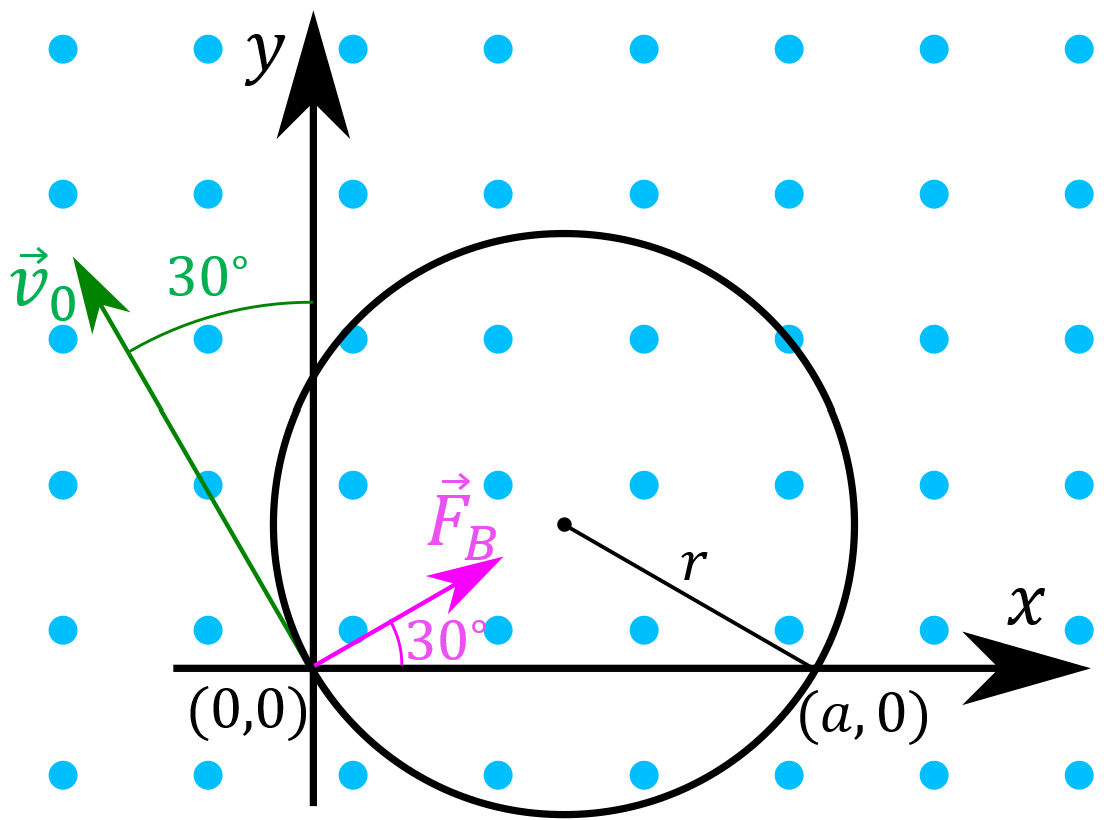
\includegraphics[width=7cm]{oz02/resources/oef-2-schets.png}
    
%     \textbf{Schets 2.1}
% \end{figure}

% \begin{enumerate}[(a)]
%     \item
%         \begin{description}[labelwidth=1.5cm, leftmargin=!]
%             \item[Gevr. :]  $ a $;
%             \item[Opl. :]   $ \vec{F} = Q \vec{v} \times \vec{B} $
                            
%                             \hspace{-0.57cm} $ \Rightarrow 
%                             ||\vec{F}_B|| = q ||\vec{v}|| \cdot ||\vec{B}|| \sin{90^{\circ}} $
                            
%                             \hspace{-0.57cm} $ \Leftrightarrow
%                             F_B = q \cdot v_0 \cdot B_0 $
                            
%                             \vspace{0.3cm}
                            
%                             $ F_B = m \cdot a_t $
                            
%                             \hspace{-0.57cm} $ \Leftrightarrow
%                             a_t = \dfrac{F}{m} 
%                             = \dfrac{q \cdot v_0 \cdot B_0}{m} $
                            
%                             \vspace{0.3cm}
                            
%                             $ a_t = \dfrac{v_0^2}{r} $
                            
%                             \hspace{-0.57cm} $ \Leftrightarrow
%                             r = \dfrac{v_0^2}{a_t} 
%                             = \dfrac{v_0^2}{\dfrac{q \cdot v_0 \cdot B_0}{m}}
%                             = \dfrac{m \cdot v_0}{q \cdot B_0} $
                            
%                             \vspace{0.3cm}
                            
%                             $ a = 2r \cdot \cos{30^{\circ}} $
%                             $ a = \sqrt{3} \dfrac{m \cdot v_0}{q \cdot B_0} $
%         \end{description}
%     \item
%         \begin{description}[labelwidth=1.5cm, leftmargin=!]
%             \item[Gevr. :]  $ t_a $;
%             \item[Opl. :]   $ a_t = r \omega^2 $
            
%                             \hspace{-0.57cm} $ \Leftrightarrow $
%                             $ \omega = \sqrt{\dfrac{a_t}{r}}
%                             = \sqrt{\dfrac{\dfrac{q \cdot v_0 \cdot B_0}{m}}{\dfrac{m \cdot v_0}{q \cdot B_0}}}
%                             = \sqrt{\dfrac{q^2 \cdot B_0^2}{m^2}}
%                             = \dfrac{q \cdot B_0}{m} $
                            
%                             \vspace{0.3cm}
                            
%                             $ \theta = 240^{\circ} = \dfrac{4}{3} \pi $ rad
                            
%                             \vspace{0.3cm}
                            
%                             $ \theta = \omega t $
                            
%                             \hspace{-0.57cm} $ \Leftrightarrow 
%                             t_a = \dfrac{\theta}{\omega}
%                             = \dfrac{\dfrac{4}{3} \pi}{\dfrac{q \cdot B_0}{m}} 
%                             = \dfrac{4}{3} \pi \dfrac{m}{q \cdot B_0} $
%         \end{description}
% \end{enumerate}

% \vspace{1cm}